\section{Experimentación con el filtro adaptativo}

En la presente sección se describe el proceso de experimentación llevado a cabo para evaluar el rendimiento del filtro adaptativo. Para la evaluación se utilizó el conjunto de prueba de la base de datos descrita en la sección \ref{sec:audio_db}.

El proceso de pruebas consistió en ingresar al filtro adaptativo señales ruidosas, obtener la respuesta del filtro y compararla con la señal original sin ruido, por medio de las métricas STOI y PESQ.

\subsection{Parámetros del filtro}

De las ecuaciones vistas en la sección \ref{sec:filtro_adaptativo_procesamiento_de_señales} se observa que antes de poder utilizar el filtro, se necesitan definir algunos parámetros:

\begin{itemize}
	\item Cantidad de coeficientes $M$.
	\item Factor de olvido $\lambda$.
	\item Factor de regularización $\epsilon$.
\end{itemize}


A continuación veremos cómo se configuraron cada uno de ellos.

\subsubsection{Cantidad de coeficientes $M$}

El parámetro M define el largo del filtro y por ende la cantidad de coeficientes. A mayor cantidad de coeficientes mayor será la capacidad del filtro para adaptarse a los retardos entre las señales captadas por los micrófonos y también será mayor la capacidad de cancelación. Sin embargo, a medida que aumentamos la cantidad de coeficientes, también aumenta el tiempo de procesamiento. Para el presente trabajo se utilizaron 16 coeficientes, es decir $M=16$.

\subsubsection{Factor de olvido $\lambda$}

El factor de olvido $\lambda$ se debe escoger en el rango $0 \ll \lambda \le 1$. En el caso extremo de $\lambda=1$, la estimación de la matriz de autocorrelación adopta el valor

\begin{equation*}
	\hat{R}_{uu} = \frac{1}{i+1} \sum_{j=0}^{i} u_j^* u_j
\end{equation*}

\noindent es decir, se promedian todas las estimaciones anteriores de $R_{uu}$. Al elegir un valor menor a uno, se dice que se le introduce memoria a la estimación ya que se le estará dando mayor importancia a las estimaciones recientes que a las pasadas. 

El parámetro $\lambda$ define la capacidad de adaptación del algoritmo. Mientras más cerca de uno esté, más lento responderá el filtro ante cambios en las características de la señal de entrada $u$. Para el presente trabajo se encontró que una buena relación de compromiso se encuentra en el valor $\lambda=0.998$.

\subsubsection{Factor de regularización $\epsilon$}

En la sección \ref{sec:adaptive_filter_rls} vimos que, desde el punto de vista de los filtros adaptativos, el filtro RLS surge de la recursión de Newton dada por:

\begin{equation}
	w_i = w_{i-1} + \mu (\epsilon I + R_{uu} )^{-1} \left( R_{du} - R_{uu} w_{i-1} \right)
\end{equation}

El término $\epsilon I$ permite regularizar la inversión de la matriz que estima $R_{uu}$, es decir regularizar la inversa de:

\begin{equation*}
	\hat{R}_{uu} = \frac{1}{i+1} \sum_{j=0}^{i} u_j^* u_j
\end{equation*}

Desarrollando la recursión y eligiendo $\epsilon(i) = \frac{\lambda^{i+1} \epsilon }{i+1}$ se obtiene que el parámetro $\epsilon$ sólo está involucrado en la condición inicial del algoritmo. Un valor usualmente utilizado y que en el presente trabajo permitió la adecuada regularización, es el de $\epsilon=0.01$


\subsection{Resultados}

\subsubsection{Medida PESQ}

Dado el conjunto de audios de prueba con un largo igual a $P$, las señales de habla ruidosas $d_p(n)$, las señales de habla sin ruido $s_p(n)$, y las señales de habla filtradas $\hat{s}_p(n)$, se definieron las siguientes medidas.

\vspace{5mm}

\noindent $\textbf{PESQ - Ruidosa}$

\vspace{5mm}

Medida PESQ entre la señal de habla ruidosa y la señal de habla sin ruido. Establece una cota inferior en la medida PESQ que debería tener la señal de habla filtrada.

\begin{equation*}
	\textbf{PESQ - Ruidosa} = \frac{1}{P-1} \sum_{p=0}^{P-1} PESQ\{ s_p(n), d_p(n) \}
\end{equation*}

\noindent $\textbf{PESQ - Filtrada}$ 

\vspace{5mm}

Medida PESQ entre la señal de habla filtrada y la señal de habla sin ruido. 

\begin{equation*}
	\textbf{PESQ - Filtrada} = \frac{1}{P-1} \sum_{p=0}^{P-1} PESQ\{ s_p(n), \hat{s}_p(n) \}
\end{equation*}

Uno de los objetivos del filtro de ruido es mejorar, o al menos mantener, la calidad de la señal de habla, es por eso que la medida PESQ calculada para la señal ruidosa $d(n)$ nos da una cota inferior, es decir se espera que:

\begin{equation*}
	\text{PESQ - Filtrada} \geq \text{PESQ - Ruidosa}
\end{equation*}

Como vimos en la sección \ref{sec:metrics}, las señales de habla ruidosa fueron construidas utilizando distintos valores de SNR. Una forma de evaluar el filtro es analizar qué tanto cambia la PESQ para cada valor de SNR utilizado.

En la figura \ref{fig:ch6_pesq_by_snr} podemos ver las medidas \textbf{PESQ - Ruidosa} y \textbf{PESQ - Filtrada} en función del nivel de ruido. En la gráfica se observa que una vez superado los $\SI{10}{dB}$, el filtro no logró mejorar la calidad de las señales de habla ruidosas, incluso genero un deterioro de la mismo.

\begin{figure}
	\centering
	\centerline{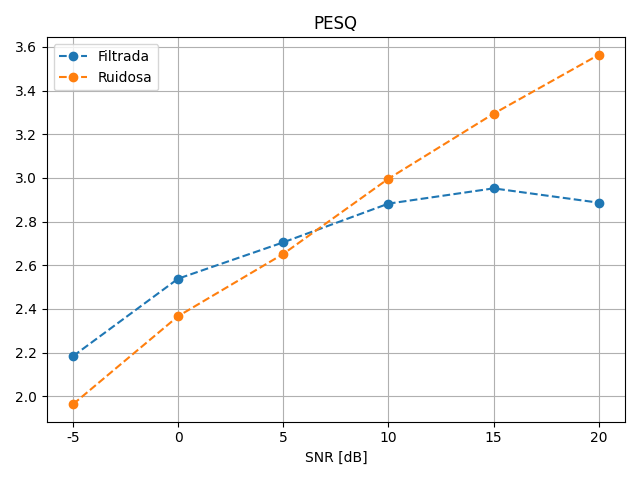
\includegraphics[scale=0.75]{images/ch6/pesq_by_snr.png}}
	\caption{PESQ en función de la SNR.}
	\label{fig:ch6_pesq_by_snr}
\end{figure}

A medida que la SNR fue aumentando, le resultó cada vez más difícil al filtro poder mejorar el valor de base de la medida $PESQ$. En la siguiente sección se analiza este comportamiento mas en detalle. En la tabla \ref{table:pesq_by_snr} podemos ver el detalle de los resultados de la figura \ref{fig:ch6_pesq_by_snr}.

\begin{table}
	\centering
	\begin{tabular}{ |c|c|c|c|c|c|c|c| } 
		\hline
		SNR [dB] & $-5$ & $0$ & $5$ & $10$ & $15$ & $20$ & Media \\ 
		\hline
		PESQ - Ruidosa & 1.22 & 1.58 & 1.99 & 2.42 & 2.82 & 3.20 & 2.20 \\
		PESQ - Filtrada & 1.57 & 1.92 & 2.19 & 2.40 & 2.48 & 2.40 & 2.16 \\
		\hline
	\end{tabular}
	\caption{PESQ en función de la SNR.}
	\label{table:pesq_by_snr}
\end{table}

Otra forma de evaluar el filtro es analizar cómo varían las medidas en función del tipo de ruido. En la figura \ref{fig:ch6_pesq_by_noise_type} podemos ver la medida PESQ en función del tipo de ruido.

\begin{figure}
	\centering
	\centerline{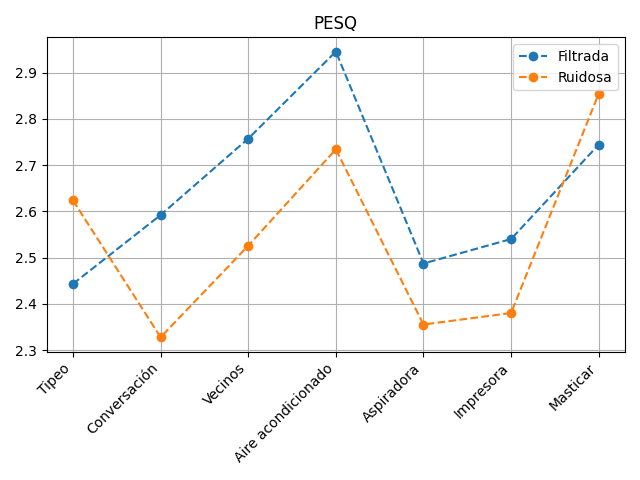
\includegraphics[scale=0.75]{images/ch6/pesq_by_noise_type.png}}
	\caption{PESQ en función del tipo de ruido.}
	\label{fig:ch6_pesq_by_noise_type}
\end{figure} 

El filtro adaptativo logró mejorar la calidad de las señales ruidosas en los tipos de ruidos; \emph{Conversación}, \emph{Vecinos}, \emph{Aspiradora} e \emph{Impresora}. Para los ruidos del tipo \emph{Tipeo} y \emph{Masticar}, la calidad disminuyó. Estos ruidos tienen la característica de ser de corta duración, lo que representa un inconveniente para el filtro adaptativo que necesita cierto tiempo para adaptarse a las nuevas condiciones de ruido y filtrarlo.

Como se observa en la tabla \ref{table:pesq_by_snr}, en valor medio, la mejora en la PESQ es pequeña y esto explica porque para algunos tipos de ruido vemos una mejora en la calidad y en otros vemos una degradación.

\subsubsection{Medida STOI}

Al igual que para la PESQ se analizaron las siguientes medidas.

\vspace{5mm}

\noindent $\textbf{STOI - Ruidosa}$

\vspace{5mm}

Medida STOI entre la señal de habla ruidosa y la señal de habla sin ruido. Establece una cota inferior en la medida STOI que debería tener la señal de habla filtrada.

\begin{equation*}
	\textbf{STOI - Ruidosa} = \frac{1}{P-1} \sum_{p=0}^{P-1} STOI\{ s_p(n), d_p(n) \}
\end{equation*}

\noindent $\textbf{STOI - Filtrada}$ 

\vspace{5mm}

Medida STOI entre la señal de habla filtrada y la señal de habla sin ruido. 

\begin{equation*}
	\textbf{STOI - Filtrada} = \frac{1}{P-1} \sum_{p=0}^{P-1} STOI\{ s_p(n), \hat{s}_p(n) \}
\end{equation*}

En la figura \ref{fig:ch6_stoi_by_snr} podemos ver las medidas \textbf{STOI - Ruidosa} y \textbf{STOI - Filtrada} en función del nivel de ruido. Al igual que para la PESQ, a partir de los $\SI{10}{dB}$ el filtro en lugar de mejorar la inteligibilidad, la empeora.  En la tabla \ref{table:stoi_by_snr} podemos ver el detalle de los resultados de la figura \ref{fig:ch6_stoi_by_snr}.

\begin{figure}
	\centering
	\centerline{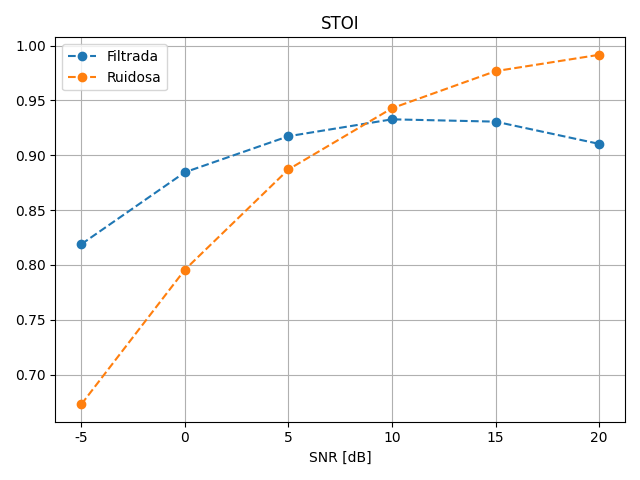
\includegraphics[scale=0.75]{images/ch6/stoi_by_snr.png}}
	\caption{STOI en función de la SNR.}
	\label{fig:ch6_stoi_by_snr}
\end{figure}

\begin{table}[ht]
	\centering
	\begin{tabular}{ |c|c|c|c|c|c|c|c| } 
		\hline
		SNR [dB] & $-5$ & $0$ & $5$ & $10$ & $15$ & $20$ & Media \\ 
		\hline
		STOI - Ruidosa & 0.67 & 0.80 & 0.89 & 0.94 & 0.97 & 0.99 & 0.88 \\
		STOI - Filtrada & 0.82 & 0.88 & 0.92 & 0.93 & 0.93 & 0.91 & 0.90 \\
		\hline
	\end{tabular}
	\caption{STOI en función de la SNR.}
	\label{table:stoi_by_snr}
\end{table}

También se analizó la medida STOI como función del tipo de ruido. En la figura \ref{fig:ch6_stoi_by_noise_type} podemos ver dicha gráfica. A diferencia de PESQ, se observa que a excepción de los ruidos del tipo \emph{Tipeo} y \emph{Masticar}, el filtro adaptativo, en promedio, logró una mejora de la inteligibilidad. La diferencia respecto a PESQ se explica mirando la figura \ref{fig:ch6_stoi_by_snr} donde podemos ver que para bajos SNRs, la mejora en la inteligibilidad es mayor que la mejora en la calidad, compensando así la degradación a altos niveles de SNR.

\begin{figure}
	\centering
	\centerline{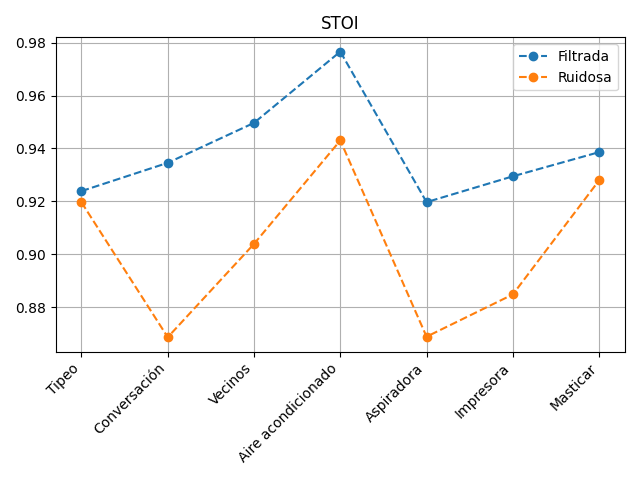
\includegraphics[scale=0.75]{images/ch6/stoi_by_noise_type.png}}
	\caption{STOI en función del tipo de ruido.}
	\label{fig:ch6_stoi_by_noise_type}
\end{figure} 

\subsubsection{Error cuadrático medio y nivel de ruido}

Dada las señales de habla sin ruido $s_p(n)$, las señales filtrada $\hat{s}_p(n)$, las señales de ruido $n_p(n)$, $N_p$ el largo de la señal $p$ y $P$ la cantidad de señales de audio en la base de datos de pruebas, se computa el error cuadrático medio, para cada uno de los niveles de ruido, como:

\begin{equation*}
	\text{ECM} = \frac{1}{P-1} \sum_{p=0}^{P} \frac{1}{N_p-1} \sum_{n=0}^{N_p} (\hat{s}_p(n) - s_p(n))^2
\end{equation*}

También definimos el nivel de ruido medio al cuadrado como:

\begin{equation*}
	\text{Nivel de ruido} = \frac{1}{P-1} \sum_{p=0}^{P} \frac{1}{N_p-1} \sum_{j=0}^{N_p} (n_p(n))^2
\end{equation*}

\begin{figure}
	\centering
	\centerline{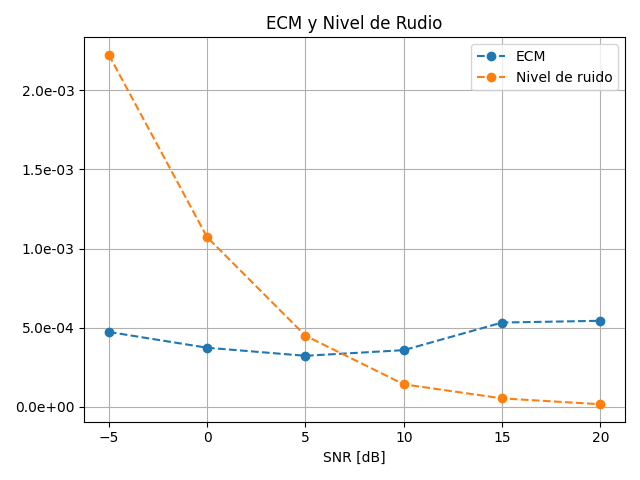
\includegraphics[scale=0.8]{images/ch6/ecm_and_noise_level.png}}
	\caption{ECM y Nivel de ruido.}
	\label{fig:ch6_mse_and_noise_level}
\end{figure}

En la figura \ref{fig:ch6_mse_and_noise_level} podemos el error cuadrático medio y el nivel de ruido como función de la SNR. En las figuras \ref{fig:ch6_pesq_by_snr} y \ref{fig:ch6_stoi_by_snr} vimos que a medida que la SNR aumentó, al filtro le resultó cada vez más difícil lograr una mejora en las medidas PESQ y STOI. 

Una explicación a este comportamiento lo podemos ver en la figura \ref{fig:ch6_mse_and_noise_level}, donde observamos que a medida que la SNR aumenta, el error cuadrático medio se vuelve comparable con el nivel ruido. Esto lleva a que las medidas  \textbf{PESQ - Filtrada} y \textbf{STOI - Filtrada} sean similares o menores que lo niveles base \textbf{PESQ - Ruidosa} y \textbf{STOI - Ruidosa}, respectivamente. En estos casos, la señal de habla filtrada tiene un nivel de ruido similar a la señal de habla ruidosa original, pero esta vez inducido por el error en estado estacionario del filtro adaptativo \cite{fundamentals_of_adaptive_filtering}.

\subsubsection{Variación de los coeficientes en función del tiempo}

Es interesante ver cómo se comportan los coeficientes del filtro para algunos ejemplos concretos. En la figura \ref{fig:ch6_variacion_temporal_de_coeficientes}  podemos ver la variación de los coeficientes del filtro en función del tiempo para 4 audios distintos. 

\begin{figure}
	\centering
	\centerline{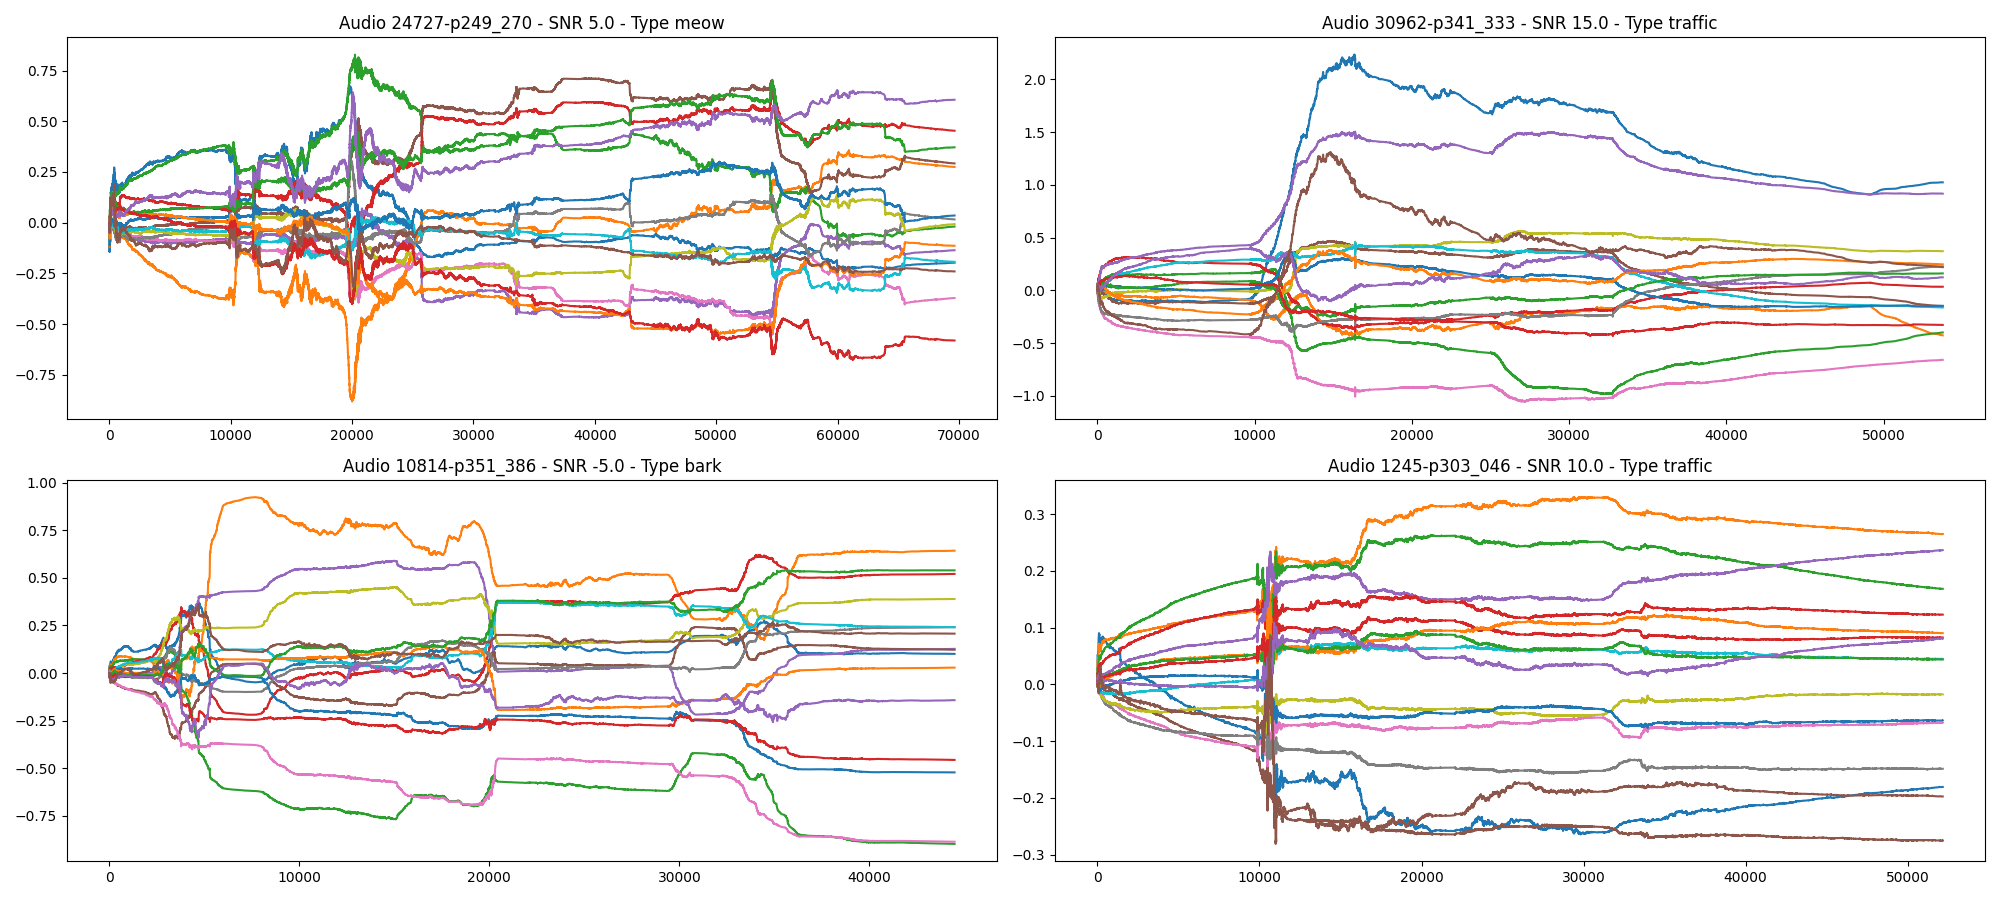
\includegraphics[scale=0.35]{images/ch6/weights.png}}
	\caption{Variación de los coeficientes en función del tiempo.}
	\label{fig:ch6_variacion_temporal_de_coeficientes}
\end{figure}

Se observa como los coeficientes se adaptan a medida que cambia la correlación entre los ruidos $n_1(n)$ y $n_2(n)$. Una vez que encuentran la nueva adaptación que minimiza el error, permanecen en un estado estacionario hasta que ocurre un nuevo cambio en el entorno.